\section{Trajectory Representation}
\label{sec:criis_graph_trajectory_representation}
\hspace{\parindent}
The CRIIS fleet coordination system represents the operating environment as a graph, as illustrated
in Figure~\ref{fig:criis_graph_environment}. Vertices correspond to decision states, while edges
represent executable actions, including robot motion and operations such as opening a door, calling
an elevator, or docking with an object~\cite{matos2025criis}. This representation allows planning
to consider both robot displacement and actions that influence the temporal coordination of the
fleet.

\begin{figure}[H]
    \centering
    
\includegraphics[width=0.8\textwidth]{criis_graph_environment.png}
    \caption{Graph representation of the operating environment~\cite{matos2025criis}.}
    \label{fig:criis_graph_environment}
\end{figure}

The graph abstracts the physical workspace into a set of vertices and directed edges, allowing the
planner to compute coordinated routes over a compact symbolic representation while the robot
controllers execute the corresponding physical trajectories.



Each vertex is associated with a unique identifier, a reference frame, a planar position, and an
orientation. The orientation value is used to define the direction of outgoing and incoming travel
edges, supporting the construction of smooth trajectories. Each edge is associated with an origin
vertex, a destination vertex, a unique identifier, a curve type, and parameters describing the
corresponding motion or action. For travel edges, the physical trajectory is encoded as a parametric
B\'ezier curve. The system also stores forward and backward execution velocities for these edges,
allowing the same geometric connection to have different temporal costs depending on the direction
of traversal.

Figure~\ref{fig:criis_parametric_edge} illustrates how the curve parameters and vertex orientations
define the shape of a travel edge between two graph vertices. This parametric representation allows
the system to generate intermediate points along each edge, producing an executable trajectory for
the robot controller.

\begin{figure}[H]
    \centering
    
\includegraphics[width=0.70\textwidth]{criis_parametric_edge.png}
    \caption{Parametric representation of a travel edge, defined from the origin and destination
    vertices, their orientations, and the curve parameters used to shape the trajectory~\cite{matos2025criis}.}
    \label{fig:criis_parametric_edge}
\end{figure}

The cost of each edge is expressed in temporal terms. For travel edges, it is computed from the
length of the corresponding parametric curve and the nominal velocity in the direction of traversal.
For actions such as docking or elevator interaction, the cost is estimated from real
execution data. This allows TEA* to reason over execution time rather than only geometric distance.

A robot plan is therefore represented as an ordered sequence of graph edges. During execution, each
robot follows this sequence locally and reports its symbolic state to the central coordination
module, typically through the current edge and the progress along it. This allows the central system
to coordinate the fleet at graph level while continuous trajectory tracking remains handled by the
robot-side control layer.

\section{System Architecture}
\label{sec:criis_system_architecture}
\hspace{\parindent}
The CRIIS fleet coordination system follows a centralized and modular architecture implemented on
top of the Robot Operating System (ROS), which provides the communication middleware between the
central coordination components and the robot-side control modules~\cite{matos2025criis}. As
illustrated in Figure~\ref{fig:criis_high_level}, the system is organized around two main parts:
the {Central Coordination Module} and the {Agent Control Module}.

The {Central Coordination Module} is responsible for global planning, supervision, and
coordination, maintaining a global view of the environment and the fleet state. In contrast, the
{Agent Control Module}, instantiated on each robot, executes the received edge sequences,
interfaces with the local navigation stack, and provides execution feedback to the central
coordination layer. This separation allows each robot to retain autonomy in localization and
low-level control, while the fleet remains coordinated through centralized planning.

\begin{figure}[H]
    \centering
    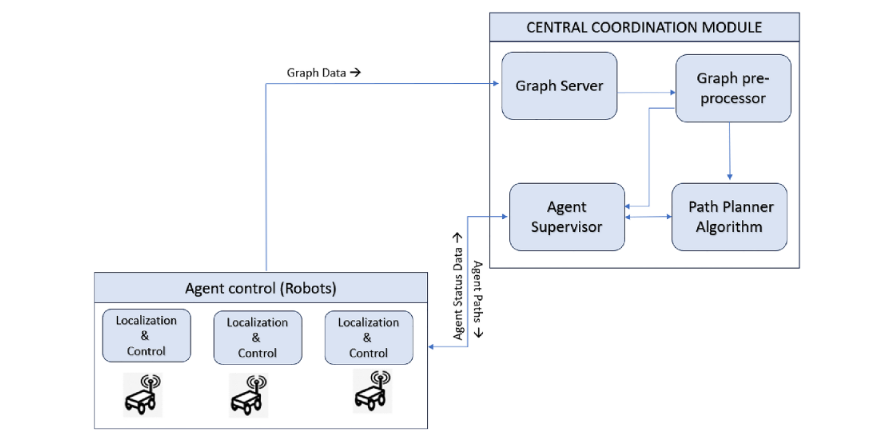
\includegraphics[width=1\textwidth]{matos.png}
    \caption{High-level architecture of the CRIIS fleet coordination system~\cite{matos2025criis}.}
    \label{fig:criis_high_level}
\end{figure}

The following subsections describe the main components involved in this coordination workflow.
The Graph Server, Graph Pre-Processor, Path Planner, and Supervisor form the central coordination
side of the system. The Navigation Handler, although not explicitly represented as an independent
block in Figure~\ref{fig:criis_high_level}, is also described because it provides the interface
between the centralized coordination logic and the robot-side navigation stack.

Figure~\ref{fig:criis_sequence_diagram} summarizes the interaction between these components during
the coordination workflow, including the exchange of planning requests, graph information, computed
paths, and execution feedback.

\begin{figure}[H]
    \centering
    
\includegraphics[width=0.95\textwidth]{seqDiagram}
    \caption{Sequence diagram of the CRIIS fleet coordination workflow.}
    \label{fig:criis_sequence_diagram}
\end{figure}

\subsection{Graph Server}
\label{subsec:graph_server}
\hspace{\parindent}
The Graph Server is responsible for storing and providing access to the global navigation graph
shared by all agents in the fleet. This graph encodes the topological structure of the environment,
including vertices, directed edges, and their associated traversal costs. In the CRIIS fleet
coordination system, these costs are expressed in temporal terms, enabling time-aware planning and
synchronization among agents~\cite{matos2025criis}.

Additionally, the Graph Server exposes a query interface that allows other components, namely the
Path Planner, to retrieve graph topology, edge attributes, and metadata required for coordination.
By decoupling graph management from planning logic, the system promotes modularity and facilitates
future extensions, such as dynamic cost updates or graph augmentation strategies.

\subsection{Graph Pre-Processor}
\label{subsec:graph_pre_processor}
\hspace{\parindent}
The Graph Pre-Processor operates during an offline configuration phase and augments the raw
navigation graph with information required for multi-robot coordination, transforming a purely
geometric representation into a coordination-aware graph~\cite{matos2025criis}. Its responsibilities
include identifying footprint-related constraints, such as parallel edges that cannot be safely
occupied simultaneously, and detecting critical shared resources, such as narrow corridors or
doorways that are prone to congestion and deadlocks.

Additionally, since TEA* advances time in discrete steps associated with edge traversals, the
pre-processor performs edge discretization and normalization according to a global temporal
resolution. This ensures consistent traversal times across the graph, improving temporal alignment
between agents and enabling more accurate space-time reasoning during planning, thereby reducing
synchronization errors and unnecessary replanning~\cite{filipe_decomposition}.

\subsection{Path Planner}
\label{subsec:path_planner}
\hspace{\parindent}
The Path Planner is the core decision-making component responsible for computing coordinated,
collision-free trajectories for the entire fleet. In the CRIIS system, this functionality is
implemented using the TEA* algorithm~\cite{matos2025criis}.

Planning requests include the current symbolic positions and target goals of all agents. Upon
receiving a request, the Path Planner retrieves the navigation graph and associated traversal costs
from the Graph Server and computes time-consistent sequences of edges for each agent. By reasoning
over a shared space-time representation, the planner can explicitly account for interactions between
agents, reserving graph resources over time and preventing conflicts through temporal exclusion
mechanisms.

The centralized nature of the Path Planner enables globally coherent solutions, particularly in
environments with shared resources or high robot density. This approach allows conflicts to be
resolved at planning time rather than during execution, reducing the likelihood of deadlocks,
emergency stops, or excessive local replanning~\cite{matos2025criis}.

\subsection{Navigation Handler}
\label{subsec:navigation_handler}
\hspace{\parindent}
The Navigation Handler serves as the integration layer between the centralized coordination logic
and the robots' low-level navigation systems. Although it is not represented as an independent
component in the high-level architecture shown in Figure~\ref{fig:criis_high_level}, it plays an
important role in the execution workflow by mediating navigation requests, plan dispatch, and
execution feedback.

In particular, the Navigation Handler exposes an API through which a robot can be requested to
navigate to a given target vertex. When this service is called, the Navigation Handler forwards the
request to the Supervisor, which in turn invokes the Path Planner to compute a feasible path within
the shared graph representation. Once the resulting plan is received, the Navigation Handler
translates the symbolic sequence of graph edges into navigation commands compatible with the
robot navigation stack.

During execution, the Navigation Handler collects feedback such as the current symbolic state,
edge completion status, and execution delays, and reports this information to the Supervisor. By
isolating execution-specific concerns from planning logic, it enhances system modularity and allows
the coordination framework to remain agnostic to the underlying robot platforms and navigation
implementations~\cite{matos2025criis}.

\subsection{Supervisor}
\label{subsec:supervisor}
\hspace{\parindent}
The Supervisor is responsible for orchestrating the overall coordination loop by closing the feedback
cycle between planning and execution. It aggregates execution feedback provided by the Navigation
Handler, monitors the progress of each agent, and maintains a global view of the system
state~\cite{matos2025criis}.

Based on this information, the Supervisor detects abnormal or unexpected conditions, such as
execution delays, deviations between planned and executed trajectories, or emerging conflicts caused
by dynamic disturbances. When such situations are identified, the Supervisor triggers replanning
requests to the Path Planner.

This supervision mechanism is a key contributor to system robustness under real-world uncertainty,
including variable execution times, communication latency, and dynamic obstacles. By enabling
adaptive replanning while preserving centralized coordination, the Supervisor ensures that the fleet
can maintain safe and efficient operation even when assumptions made at planning time are
violated~\cite{matos2025criis}.

\section{Summary}
\label{sec:criis_system_summary}
\hspace{\parindent}
This chapter described the existing CRIIS fleet coordination system used as the reference
architecture for this dissertation. First, the graph and trajectory representation adopted by the
system was presented, highlighting how vertices define decision states and edges encode executable
actions, including both travel motions and operations not directly related to navigation. The use of
temporal edge costs allows TEA* to reason over execution time, while robot plans are represented as
ordered sequences of graph edges.

The chapter then introduced the modular architecture of the system, implemented in ROS, and
distinguished between the Central Coordination Module and the Agent Control Module. The main
components involved in the coordination workflow were then described, including the Graph Server,
Graph Pre-Processor, Path Planner, Navigation Handler, and Supervisor. Although the Navigation
Handler is not represented as an independent block in the high-level architecture, it was included
because it provides the interface between centralized coordination and robot-side navigation. This
architecture provides the foundation upon which the prioritization heuristics, parallel planning
framework, and batching mechanisms developed in the following chapters are introduced.
